\section{Results}

The performance of the proposed models has been assessed across various configurations to leverage their capabilities. The outcomes for each model are presented in the subsequent sections, categorized by model. The results for the baseline are reported in the concluding section dedicated to the comparison, as this model do not have specific configurations.

\subsection{LSTM Model}

This is the slowest algorithm, as the evaluation of each individual in the population involves training a LSTM model for a specified number of epochs—set to $15$ in this instance. The initial population consists of $20$ randomly initialized individuals, and the algorithm runs for $30$ generations. The tournament size $K$ is set to $3$ and the number of elites preserved at each generation is set to $2$. The crossover rate $p_c$ and mutation rate $p_m$ are respectively set to $p_c=0.3$ and $p_m=0.7$. The entire experiment takes several minutes, and the fitness progress over the generations is depicted in Figure \ref{fig:fitness-lstm}, where the plot illustrates the best model's fitness evaluated on the validation set at the end of each generation.

\begin{figure}[h]
\centering
    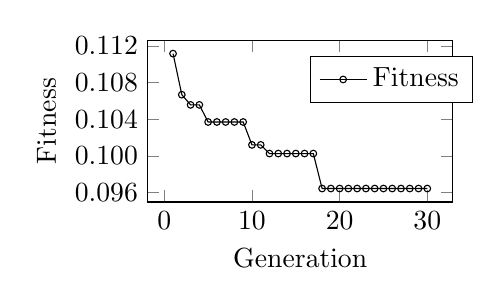
\begin{tikzpicture}
      \begin{axis}[
        xlabel={Generation},
        ylabel={Fitness},
        width=0.45\textwidth,
        height=0.3\textwidth,
        legend style={at={(0.8, 0.9)},anchor=north},
        mark size=1.2,
        y tick label style={/pgf/number format/.cd,fixed,fixed zerofill=true,precision=3},
        ytick={0.096,0.100,...,0.12},
      ]
      
      \addplot[mark=o] coordinates {
        (1, 0.111149)
        (2, 0.106667)
        (3, 0.105555)
        (4, 0.105555)
        (5, 0.103689)
        (6, 0.103689)
        (7, 0.103689)
        (8, 0.103689)
        (9, 0.103689)
        (10, 0.101192)
        (11, 0.101192)
        (12, 0.100245)
        (13, 0.100245)
        (14, 0.100245)
        (15, 0.100245)
        (16, 0.100245)
        (17, 0.100245)
        (18, 0.096430)
        (19, 0.096430)
        (20, 0.096430)
        (21, 0.096430)
        (22, 0.096430)
        (23, 0.096430)
        (24, 0.096430)
        (25, 0.096430)
        (26, 0.096430)
        (27, 0.096430)
        (28, 0.096430)
        (29, 0.096430)
        (30, 0.096430)
      };
      
      \legend{Fitness}
      \end{axis}
    
    \end{tikzpicture}
\caption{Change in fitness over generations.} 
\label{fig:fitness-lstm}
\end{figure}

The best individual reported by Genetic Algorithms has a fitness of $0.0984$ on the validation set, and the optimal configuration found is \verb|[61, 33, 1, 0.0044261263, []]|. Interestingly, the model did not incorporate any additional weather parameters beyond the outdoor temperature, indicating that these omitted parameters may not have played a crucial role in the forecasting process.

\subsection{Genetic Programming}

In this particular case, the problem space is large, necessitating a substantial population. Specifically, the population size is configured with $500$ individuals, and the tournament size $K$ is set to $5$. A range of values for the crossover rate $p_c$ and mutation rate $p_m$ has been explored, yielding notably diverse outcomes. The optimal tree is derived with $p_c=0.8$ and $p_m=0.1$, executing over a span of $20$ generations. The visual representation of the evolved tree is provided in Figure \ref{fig:gp-tree}, where $\{x_0, x_1, x_2, x_3\}$ denotes the past $p=4$, with $x_3$ being the latest one, and $e_0=0.17488$ and $e_1=0.97058$ represent ephemeral variables. The fitness progress over the generations is depicted in Figure \ref{fig:gp-evolution}, where the plot illustrates the best model’s fitness evaluated
on the training set at the end of each generation as well as the average size of the evolved trees.

An interesting observation arises from the evolved tree structure: only the initial and final temperature observations are employed to forecast the temperature of the next hour while the intermediate measurements of the temperature are disregarded in this predictive process. This distinctive characteristic adds nuance to the understanding of how the Genetic Programming model interprets and utilizes past observations and ephemeral variables in forecasting.

\begin{figure}[h]
\centering
    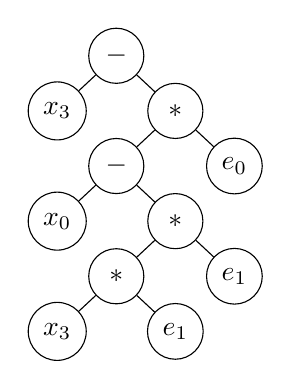
\begin{tikzpicture}[
      every node/.style={circle, draw, minimum size=7mm},
      level distance=7mm,
      sibling distance=15mm,
    ]
    \node {$-$}
      child {node {$x_3$}}
      child {node {$*$}
        child {node {$-$}
          child {node {$x_0$}}
          child {node {$*$}
            child {node {$*$}
              child {node {$x_3$}}
              child {node {$e_1$}}
            }
            child {node {$e_1$}}
          }
        }
        child {node {$e_0$}}
      };
    \end{tikzpicture}    
\caption{Evolved tree generated by Genetic Programming.} 
\label{fig:gp-tree}
\end{figure}


\begin{figure}
    \centering
    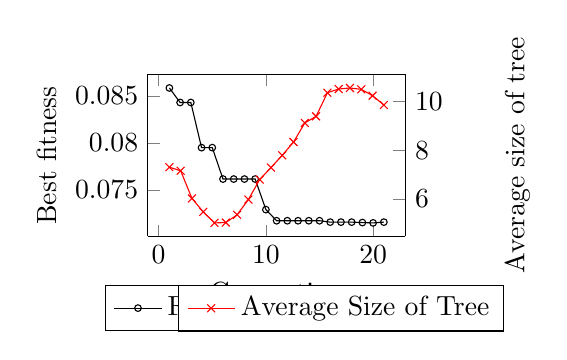
\begin{tikzpicture}
    
      \begin{axis}[
        xlabel={Generation},
        ylabel={Best fitness},
        axis y line*=left,
        legend style={at={(0.15,-0.3)}, anchor=north, legend columns=-1},
        yticklabel style={
            /pgf/number format/fixed,
            /pgf/number format/precision=5
        },
        width=0.4\textwidth,
        height=0.3\textwidth,
        scaled y ticks=false,
        mark size=1.2,
      ]
      
      \addplot[mark=o, black] coordinates {
          (1, 0.08584692178901428)
          (2, 0.08430659472942352)
          (3, 0.08430659472942352)
          (4, 0.07950782254907311)
          (5, 0.07950782254907311)
          (6, 0.07617175246263186)
          (7, 0.07617175246263186)
          (8, 0.07617175246263186)
          (9, 0.07617175246263186)
          (10, 0.07292518568784243)
          (11, 0.07174215158304403)
          (12, 0.07174215158304403)
          (13, 0.07174215158304403)
          (14, 0.07174215158304403)
          (15, 0.07174215158304403)
          (16, 0.07159554874702596)
          (17, 0.07159554874702596)
          (18, 0.07159554874702596)
          (19, 0.07154947389260462)
          (20, 0.07151369182701221)
          (21, 0.07159554874702596)
      };
      
      \legend{Fitness}
      
      \end{axis}
      
      \begin{axis}[
        axis x line=none,
        axis y line*=right,
        ylabel={Average size of tree},
        y label style={at={(1.35,0.5)}},
        legend style={at={(0.75,-0.3)}, anchor=north, legend columns=-1},
        width=0.4\textwidth,
        height=0.3\textwidth,
      ]
      
      \addplot[mark=x, red] coordinates {
          (1, 7.308)
          (2, 7.16)
          (3, 6.024)
          (4, 5.472)
          (5, 5.018)
          (6, 5.032)
          (7, 5.35)
          (8, 5.978)
          (9, 6.8)
          (10, 7.292)
          (11, 7.796)
          (12, 8.342)
          (13, 9.128)
          (14, 9.398)
          (15, 10.37)
          (16, 10.52)
          (17, 10.564)
          (18, 10.508)
          (19, 10.248)
          (20, 9.864)
      };
      
      \legend{Average Size of Tree}
      
      \end{axis}
    \end{tikzpicture}

\caption{Fitness trend and average tree size over generations.} 
\label{fig:gp-evolution}
\end{figure}

\subsection{Comparison}

All the three models were tested on the test split of the dataset, containing the data of the last half of the year, obtaining the results reported in Table \ref{results}. The results detailed in Table \ref{results}, distinctly demonstrate the LSTM-based model's superior performance in terms of Mean Absolute Error. However, in terms of complexity, Genetic Programming produced an interpretable model for the given problem, characterized by basic arithmetic operations. In contrast, the LSTM model involved a more intricate structure with a total of $3501$ parameters.

\begin{table}[htbp]
  \centering
  \begin{tabular}{lccc}
    \toprule
     & \textbf{Baseline} & \textbf{LSTM} & \textbf{GP} \\
    \midrule
    \textbf{MAE} & 0.1126 & 0.08005 & 0.0929 \\
    \bottomrule
  \end{tabular}
  \caption{MAE values for different models}
  \label{results}
\end{table}